\Subsection{Собственные интегралы с параметрами}

\begin{statement}
    $(X, \mathcal{A}, \mu)$ -- пр-во с мерой, $T$ -- метрическое пр-во, $f: X \times T \rightarrow \tilde{\mathbb{R}}, \ \forall t \in T, \ E_t \in \mathcal{A}, \ f(\cdot, t)$ -- измеримая.

    $F(t) := \int_{E_t} {f(x, t) d \mu(x)}$.

    \begin{enumerate}
        \item {
            $t_0$ -- предельная точка.

            $\forall x \ f(x, t) \underbrace{\rightarrow}_{t \rightarrow t_0} \dots \underbrace{\implies}_{?} F(t) \underbrace{\rightarrow}_{t \rightarrow t_0}$
        }
        \item {
            $f(x, t)$ непрер. в точке $t_0, \ \forall x \underbrace{\implies}_{?} F$ непрер. в $t_0$.
        }
        \item {
            $f(x, t)$ дифф. по $t, \ \forall x \underbrace{\implies}_{?} F$ дифф., какая формула для производной?
        }
        \item {
            Если $\nu$ -- мера на $T$. $\int_T {F(t) d \nu (t)} = \int_{T} { \int_{E_t} { f(x, t) d \mu(x) d \nu (t) } } = \int_T { \int_X { \mathds{1}_{E_t} (x) \cdot f(x, t) d \mu (x) d \nu (t) } }$
        }
    \end{enumerate}
\end{statement}
\begin{theorem}
    $t_0$ -- предельная точка $T$. $f(\cdot, t)$ -- суммируема $\forall t \in T$, $g(x) := \lim_{t \rightarrow t_0} { f(x, t) }$.

    \textbf{Локальное условие Лебега:}

    Пусть найдется окр-ть $U_{t_0}$ и суммир. ф-я $\Phi: X \rightarrow \overline{\mathbb{R}}$, т.ч. $|f(x, t)| \leq \Phi(x) \ \forall t \in U_{t_0}$.

    Тогда $\lim_{t \rightarrow t_0} { \left(\int_{X}{f(x, t) d \mu(x)}\right) } = \int_{X} { g(x) d \mu(x) }$.
\end{theorem}

\begin{proof}
    Проверяем по Гейне. Берем $t_n \rightarrow t_0, \ f_n(x) := f(x, t_n)$, $\Phi(x) \geq | f(x, t_n) | = |f_n(x)|$ при больших $n$.

    $\underbrace{\implies}_{\text{т. Лебега}} \lim_{n \rightarrow \infty} { \int_{X} { f_n (x) d \mu (x) } } = \int_{X} { \underbrace{\lim_{n \rightarrow \infty} {f_n(x)}}_{= g(x)} d \mu (x)}$
\end{proof}

\begin{definition}
    $f: X \times T \rightarrow \mathbb{R}, \ g: X \rightarrow \mathbb{R}$, $t_0$ -- предельная точка $T$, $f(x, t) \underbrace{\rightrightarrows}_{t \rightarrow t_0} g(x)$, если $\forall \epsilon > 0 \ \exists \delta > 0, \ \forall t \in T: \ \rho_T (t, t_0) < \delta, \ \forall x \in X: \ | f(x, t) - g(x) | < \epsilon$.
\end{definition}

\begin{remark}
    $f(x, t) \underbrace{\rightrightarrows}_{t \rightarrow t_0} g(x) \Leftrightarrow \sup_{x \in X} { | f(x, t) - g(x) | } \underbrace{\rightarrow}_{t \rightarrow t_0} 0$
\end{remark}

\begin{consequence}
    Если $\mu X < +\infty, \ f(x, t) \underbrace{\rightrightarrows}_{t \rightarrow t_0} g(x)$, то $\int_X { f(x, t) d \mu(x) } \underbrace{\rightarrow}_{t \rightarrow t_0} \int_X { g d \mu }$ и $g$ -- суммируемая ф-я.
\end{consequence}

\begin{proof}
    При $t$ близких к $t_0$: $|f(x, t) - g(x)| \leq 1 \implies$ берем $t_1$, для которого верно $|f(x, t_1) - g(x)| \leq 1 \implies |g(x)| \leq 1 + |f(x, t_1)|$ -- суммируема $\implies$ при $t$ близких к $t_0: $ $|f(x, t)| \leq 1 + |g(x)|$ -- суммир.
\end{proof}

\begin{remark}
    Условие $\mu X < +\infty$ существенно.

    $X = [0, +\infty), \ \mu = \lambda_1, \ f_n(x) = \frac{1}{n} \mathds{1}_{[0, n]} (x) \rightrightarrows 0$,

    $\int_{[0, +\infty)} {f_n d \lambda_1} = 1$.
\end{remark}

\begin{consequence}
    $f(x, t)$ непрер. в точке $t_0$, $\forall x \in X$ и существует суммир. $\Phi(x)$, т.ч. $| f(x, t) | \leq \Phi(x)$ при $t$ близких к $t_0, \ \forall x \in X$. 

    Тогда $F(t) = \int_X{ f(x, t) d \mu (x) }$ непрер. в точке $t_0$.
\end{consequence}
\begin{proof}
    $\lim_{t \rightarrow t_0} { f(x, t) } = f(x, t_0)$ и подставляем в теорему.
\end{proof}

\begin{lemma}
    Декартово произведение компактов -- компакт.

    $(X, \rho), \ (Y, d)$ -- метрические про-ва. $A \subset X, \ B \subset Y$ -- компакты.

    Тогда $A \times B$ -- компакт в $(X \times Y, r)$, $r\left((x, y), (x', y')\right) = \rho(x, x') + d(y, y')$
\end{lemma}
\begin{proof}
    Проверяем секвенциальную компактность.

    $x_n \in A, \ y_n \in B, \ (x_n, y_n)$

    хотим выбрать сх-ся подпосл. Выбираем $x_{n_k}$, т.ч. она сходится, а затем из $y_{n_k}$ подпосл $y_{n_{k_j}}$, которая сх-ся.

    Тогда $(x_{n_{k_j}}, y_{n_{k_j}})$ сх-ся покоординатно $\implies$ сх-ся по метрике $r$.
\end{proof}

\begin{theorem}
    $\mu X < +\infty$, $X$ и $T$ -- компакты, $f \in C(X \times T)$. Тогда $F(t) = \int_{X} {f(x, t)d \mu(x)} \in C(T)$. 
\end{theorem}
\begin{proof}
    $f$ -- непр-на на компакте $\implies$ ограничена $\implies$ $| f(x, t) | \leq M$ -- суммир. мажоранта.
\end{proof}
\begin{consequence}
    Если $\mu X < +\infty$, $X$ -- компакт, $\Omega \subset \mathbb{R}^m$ открытое, $f \in C(X \times \Omega)$.

    Тогда $F(t) = \int_{X} {f(x, t) d \mu(x)} \in C(\Omega)$.
\end{consequence}
\begin{proof}
    Берем $a \in \Omega$. Хотим проверить непрер. в точке $a$.

    Возьмем $\overline{B}_r(a) \subset \Omega$ -- компакт $\implies f \in C(X \times \overline{B}_r(a))$

    % todo: picture

    $\implies F \in C(\overline{B}_r(a)) \implies F$ непрер. в точке $a$.
\end{proof}

\begin{theorem}
    $T \subset \mathbb{R}$ промежуток, $f : X \times T \rightarrow \mathbb{R}, \ f'_t (x, t)$ существ. $\forall x \in X, \ \forall t \in T$ и $f'_t(x, t)$ удовлетворяет \textbf{локальным условиям Лебега} в точке $t_0$.

    Тогда $F$ -- дифф. в точке $t_0$ и $F'(t_0) = \int_X { f'_t (x, t_0) d \mu (x) }$. 
\end{theorem}
\begin{proof}
    $\frac{F(t_0 + h) - F(t_0)}{h} = \int_X {\underbrace{\frac{f(x, t_0 + h) - f(x, t_0)}{h}}_{=: g(x, h)}}d \mu (x)$.

    Нужно локальное условие Лебега для $g(x, h)$.

    $f(x, t_0 + h) - f(x, t_0) = h \cdot f'_t(x, t_0 + \theta_h \cdot h)$

    $g(x, h) = f'_t(x, t_0 + \theta_h \cdot h)$

    Знаем, что $\exists U_{t_0}$, т.ч. $| f'_t(x, t) | \leq \Phi(x)$ -- суммир. $\ \forall x, \forall t \in U_{t_0}$.

    Рассмотрим $|| h || < \epsilon$, т.ч. $t_0 + h \in U_{t_0}$
    
    % todo: picture

    $\implies t_0 + \theta_h \cdot h \in U_{t_0} \implies | f'_t(x, t_0 + \theta_h h) | = |g(x, h)| \leq \Phi(x) \implies $ можно переходить к пределу под знаком интеграла, а предел $\lim_{h \rightarrow 0} {g(x, h)} = f'_t(x, t_0)$.
\end{proof}

\begin{consequence}
    $T \subset \mathbb{R}$ -- отрезок, $X$ -- компакт, $\mu X < +\infty$, $f, f'_t \in C(X \times T)$.

    Тогда $F \in C^1(T)$ и $F'(t) = \int_X{f'_t (x, t) d \mu (x)}$.
\end{consequence}

\begin{proof}
    $f'_t$ -- непр. на компакте $\implies$ ограничена $\implies | f'_t(x, t) | \leq M$ -- сумм. мажоранта.
\end{proof}



\begin{theorem}
    \textbf{Формула Лейбница}.

    $f: \underbrace{[a, b]}_{x} \times \underbrace{[c, d]}_{t} \rightarrow \mathbb{R}$, $f, f'_t \in C([a, b] \times [c, d]), \ \phi, \psi : [c, d] \rightarrow [a, b]$ непр. дифф.

    $F(t) := \int_{\phi(t)}^{\psi(t)} { f(x, t) d x }$.

    Тогда $F$ -- дифф. и $F'(t) = \int_{\phi(t)}^{\psi(t)} { f'_t (x, t) dx } + f (\psi(t), t) \cdot \psi'(t) - f(\phi(t), t) \cdot \phi'(t)$.
\end{theorem}
\begin{proof}
    $\Phi(\alpha, \beta, t) = \int_{\alpha}^{\beta} {f(x, t) d x}$.

    $\frac{d\Phi}{d \beta} = f(\beta, t)$ -- непр. по условию
    
    $\frac{d\Phi}{d \alpha} = -f(\alpha, t)$ -- непр.

    $\frac{d \Phi}{d t} = \int_{\alpha}^{\beta} {f'_t (x, t) d x}$ -- непр.

    Так как все частные производные непр., то $\Phi$ -- дифф.

    $F(t) = \Phi(\phi(t), \psi(t), t) \implies F'(t) = \frac{d \Phi}{d \alpha} \phi'(t) + \frac{d \Phi}{d \beta} \psi'(t) + \frac{d\Phi}{dt}$.
\end{proof}

\begin{example}
    $F(t) := \int_{0}^{+\infty} {e^{-x^2} \cdot \cos(tx) dx}$

    Так как есть локальное условие Лебега (на самом деле $\int_{0}^{+\infty} { x e^{-x^2} d x } < +\infty$):

    $F'(t) = -\int_{0}^{+\infty} { e^{-x^2} \sin(tx) \cdot x dx } = \frac{1}{2} \cdot \int_{0}^{+\infty} { \sin(tx) \cdot d (e^{-x^2}) } = \frac{1}{2} \cdot e^{-x^2} \sin(tx) |_{0}^{+\infty} - \frac{1}{2} \cdot \int_{0}^{+\infty} { t \cos{tx} e^{-x^2} dx }$.

    $F'(t) = -\frac{1}{2} t F(t)$.
    
    $\underbrace{\frac{F'}{F}}_{= \ (\ln{F})'} = -\frac{t}{2} \implies \ln{F} = -\frac{t^2}{4} + C_0 \implies F(t) = C \cdot e^{\frac{-t^2}{4}}$.

    $F(t) e^{\frac{t^2}{4}} = C$.

    Более строго:

    $\left( F(t) e^{\frac{t^2}{4}} \right)' = F' e^{\frac{t^2}{4}} + F \cdot \frac{t}{2} e^{\frac{t^2}{4}} = e^{\frac{t^2}{4}} \cdot \underbrace{(F' + \frac{t}{2} \cdot F)}_{= 0} = 0$.

    Хотим узнать константу:

    $F(0) = \int_{0}^{+\infty} { e^{-x^2} dx } = \frac{\sqrt{\pi}}{2}$

    $F(t) = \frac{\sqrt{\pi}}{2} \cdot e^{\frac{-t^2}{4}}$.
\end{example}



\Subsection{Несобственные интегралы с параметрами}

$F(t) := \int_{a}^{+\infty} { f(x, t) dx }: \ \forall t \in T$ интеграл сх-ся.

\begin{definition}
    $\int_{a}^{+\infty} { f(x, t) dx }$ -- равномерно сх-ся, если $\forall \epsilon > 0 \ \exists B \ \forall b > B \ \forall t \in T: \ | \int_{b}^{+\infty} { f(x, t) d x } | < \epsilon$
\end{definition}

\begin{remark}
    $F_b(t) := \int_{a}^{b} { f(x, t) dx }$.

    $\int_{a}^{+\infty} { \dots }$ -- равном сх-ся $\Leftrightarrow F_b \underbrace{\rightrightarrows}_{b \rightarrow +\infty} F$ равном. по $t \in T$.
\end{remark}
\begin{proof}
    $\forall \epsilon > 0 \ \exists B \ \forall b > B \ \forall t \in T: \ \underbrace{| F_b(t) - F(t) |}_{= -\int_{b}^{+\infty} { f(x, t) d x }} < \epsilon$
\end{proof}

\begin{example}
    $\int_{0}^{+\infty} { e^{-tx} dx }, \ t > 0$

    $\int_{b}^{+\infty} { e^{-tx} dx } = -\frac{e^{-tx}}{t} |_{x=b}^{x=+\infty} = \frac{e^{-bt}}{t}$.

    \begin{enumerate}
        \item {
            $t \geq t_0 > 0:$

            $\frac{e^{-bt}}{t} \leq \frac{e^{-bt_0}}{t_0} < \epsilon$
        }
        \item {
            $t > 0:$

            $\frac{e^{-bt}}{t} \underbrace{\rightarrow}_{t \rightarrow 0+} +\infty \implies$ нет равномерной сх-ти.
        }
    \end{enumerate}
\end{example}

\begin{theorem}
    \textbf{Критерий Коши}.

    $\int_{a}^{+\infty} { f(x, t) dx }$ равн. сх-ся $\Leftrightarrow \forall \epsilon > 0 \ \exists B \ \forall b, c > B \ \forall t \in T: \ | \int_b^{c} { f(x, t) d x } | < \epsilon$.
\end{theorem}
\begin{proof}
    $ \int_{a}^{+\infty} { f(x, t) dx } $ равн. сх-ся $\Leftrightarrow$
    
    $\Leftrightarrow F_b \rightrightarrows F \ (\text{где } F_b(t) = \int_{a}^{b} {f(x, t) dx}, \ F(t) = \int_{a}^{+\infty} {f(x, t) dx}) \Leftrightarrow$ 
    
    $\Leftrightarrow \forall \epsilon > 0 \ \exists B \ \forall b, c > B \ \forall t \in T: \ \underbrace{| F_b(t) - F_c(t) |}_{\int_{b}^{c} { f(x, t) d x }} < \epsilon$.
\end{proof}

\begin{consequence}
    $f: [a, +\infty) \times [c, d] \rightarrow \mathbb{R}$ непрерывная.

    $ F(t) = \int_{a}^{+\infty} { f(x, t) d x } $ сх-ся $\forall t \in (c, d)$ и расх-ся при $t=c$ или $t=d$.

    Тогда сходимость неравномерная.
\end{consequence}
\begin{proof}
    Пусть $\int_{a}^{+\infty}$ сх-ся равномерно $\implies$:

    по Критерию Коши и тому, что $f$ непр. на $[b, b'] \times [c, d]$:


    $\forall \epsilon > 0 \ \exists B > a \ \forall b, b' > B \ \forall t \in (c, d): \ \underbrace{\left| \int_{b}^{b'} { f(x, t) d x } \right|}_{\rightarrow \int_{b}^{b'} { f(x, c) d x } \text{, при } t \rightarrow c} < \epsilon \implies$

    $\implies \forall \epsilon > 0 \ \exists B > a \ \forall b, b' > B \ \left| \int_{b}^{b'} { f(x, c) dx } \right| \leq \epsilon \underbrace{\implies}_{\text{критерий Коши}} \int_{a}^{+\infty} { f(x, c) dx }$ сх-ся $\implies$ противоречие.
\end{proof}

\begin{example}
    $\int_{0}^{+\infty} { e^{-tx^2} dx }, \ t > 0$ сх-ся неравномерно, так как при $t = 0$ расходится.
\end{example}

\begin{theorem}
    \textbf{Признак Вейерштрасса}.

    $f, g: [a, +\infty) \times T \rightarrow \mathbb{R}$ и $|f(x, t)| \leq g(x, t): \ \forall x \geq a, \ \forall t \in T$.

    Если $\int_{a}^{+\infty} { g(x, t) dx }$ равном. сх-ся, то $\int_{a}^{+\infty} { f(x, t) dx }$ равн. сх-ся.
\end{theorem}
\begin{proof}
    Пишем критерий Коши для $\int_{a}^{+\infty} { g(x, t) dx }$:

    $\forall \epsilon > 0 \ \exists B \ \forall b, c > B: \ \underbrace{\int_{b}^{c} { g(x, t) dx }}_{< \epsilon} \geq \int_{b}^{c} { |f(x, t)| dx } \geq \left| \int_{b}^{c} { f(x, t) d x } \right|$
\end{proof}

\begin{consequence}
    Если $\left| f(x, t) \right| \leq g(x) \ \forall x \geq a, \ \forall t \in T$ и $\int_{a}^{+\infty} { g(x) dx }$ сх-ся, то $\int_{a}^{+\infty} { f(x, t) dx }$ сх-ся равномерно.
\end{consequence}
\begin{example}
    $\int_{0}^{+\infty} { \frac{\cos(xt)}{x^2 + 1} dx }$ равн. сх-ся при $t \in \mathbb{R}$.

    $\left| \frac{\cos(xt)}{x^2 + 1} \right| \leq \frac{1}{x^2 + 1}$ и $\int_0^{+\infty} { \frac{dx}{x^2+1} } < +\infty$.
\end{example}

\begin{theorem}
    \textbf{Признак Дирихле}.

    $\int_{a}^{+\infty} { f(x, t) g(x, t) d x }$.

    Пусть

    \begin{enumerate}
        \item {
            $\exists M: \ \forall b > a, \ \forall t \in T: \ \left| \int_{a}^{b} { f(x, t) dx } \right| \leq M$
        }
        \item {
            $g$ монотонна по $x: \ \forall t \in T$.
        }
        \item {
            $g \underbrace{\rightrightarrows}_{x \rightarrow +\infty} 0$
        }
    \end{enumerate}

    Тогда $\int_{a}^{+\infty} { f(x, t) g(x, t) d x }$ равномерно сх-ся.
\end{theorem}

\begin{proof}
    Для дифф. ф-й $g$:

    $F(y, t) = \int_{a}^{y} { f(x, t) dx }$.

    $(1) \Rightarrow |F(y, t)| \leq M: \ \forall y, \ \forall t$.

    $\int_{a}^{y} { f(x, t) g(x, t) dx } = \underbrace{F(x, t) g(x, t)|_{x=a}^{x=y}}_{= F(y, t) g(y, t)} - \int_{a}^{y} { F(x, t) g'_x(x, t) d x }$

    $\left| F(y, t) g(y, t) \right| \leq M | g(y, t) | \underbrace{\rightrightarrows}_{y \rightarrow +\infty} 0$

    $ \int_{a}^{+\infty} { F(x, t) g'_x(x, t) d x } $ -- равном. сх-ся.

    $|F(x, t) g'_x(x, t)| \leq M | g'_x(x, t) |$.

    Надо доказать, что $\int_{a}^{+\infty} { | g'_x (x, t) | dx }$ равн. сх-ся.

    $\int_{a}^{y} { | g'_x (x, t) | dx } = \left| \int_{a}^{y} { g'_x (x, t) dx } \right| = \left| g(x, t)|_{x=a}^{x=y} \right| = | \underbrace{g(y, t)}_{\rightrightarrows 0 \text{ по усл.}} - g(a, t) | \rightrightarrows |g(a, t)|$.

    % Тут какие-то слова, почему все получилось (у меня мозг поплыл).
\end{proof}

\begin{theorem}
    \textbf{Признак Абеля}.

    $\int_{a}^{+\infty} { f(x, t) g(x, t) dx }$. Пусть 
    
    \begin{enumerate}
        \item {
            $\int_{a}^{+\infty} { f(x, t) dx }$ равн. сх-ся.
        }
        \item {
            $g$ монотонна по $x: \ \forall t \in T$. 
        }
        \item {
            $| g(x, t) | \leq M, \ \forall x \geq a, \ \forall t \in T$
        }
    \end{enumerate}

    Тогда $\int_{a}^{+\infty} { f(x, t) g(x, t) dx }$ равном. сх-ся.
\end{theorem}
\begin{proof}
    Для дифф. ф-й $g$:

    $F_b (y, t) = \int_{b}^{y} { f(x, t) dx }$

    $\int_{b}^{c} { f(x, t) g(x, t) dx } = \underbrace{F_b (x, t) g(x, t) |_{x=b}^{x=c}}_{= F_b(c, t) g(c, t)} - \int_b^{c} { F_b(x, t) g'_x(x, t) dx }$

    Применим крит. Коши для $\int_{a}^{+\infty} {f(x, t) dx}$:
    
    $\exists B : \ \forall y, b > B \ \forall t \in T: \ \left| F_b(y, t)  \right| < \epsilon$, смотрим на $b > B \implies |F_b(x, t)| < \epsilon$.

    $|F_b(c, t) g(c, t)| < \epsilon \cdot M$.

    $\left| \int_{b}^{c} { F_b(x, t) g'_x(x, t) dx } \right| \leq \int_{b}^{c} { \underbrace{|F_b(x, t)|}_{< \epsilon} |g'_x(x, t)| dx} < \epsilon \cdot \int_{b}^{c} { g'_x(x, t) dx } = \epsilon \left| \int_{b}^{c} { g'_x(x, t) d x } \right| =$
    
    $= \epsilon \left| g(x, t)|_{x=b}^{x=c}  \right| \leq \epsilon \cdot 2 M$.

    Получается, что оценили $\int_{b}^{c} { f(x, t) g(x, t) dx } < 3 \epsilon M$, то есть проверили критерий Коши для исходного интеграла.
\end{proof}
\begin{example}
    $\int_{1}^{+\infty} { \frac{\sin(x)}{x^t} dx }, \ t > 0$.

    \begin{enumerate}
        \item {
            $t \geq t_0 > 0$. Дирихле: $f(x, t) = \sin(x), \ g(x, t) = \frac{1}{x^t}$ -- вторая монотонно убывает.

            $\left| \int_{1}^{b} { \sin(x) dx } \right| \leq 2$.

            $g(x, t) \rightrightarrows 0$: $|g(x, t)| = \frac{1}{x^t} \leq \frac{1}{x^{t_0}} \underbrace{\rightarrow}_{x \rightarrow +\infty} 0$.

            Есть равн. сх-ть.
        }
        \item {
            $t > 0$. Нет равн. сх-ти, так как расх-ся при $t=0$.
        }
    \end{enumerate}
\end{example}

\begin{theorem}
    $f: [a, +\infty) \times T \rightarrow \mathbb{R}, \ t_0$ -- предельная точка $T$.

    Если
    \begin{enumerate}
        \item {
            $\int_{a}^{+\infty} { f(x, t) dx }$ равномерно сх-ся (по $t \in T$).
        }
        \item {
            $f(x, t) \underbrace{\rightrightarrows}_{t \rightarrow t_0} \phi(x)$ равномер. по $x$ на любом конечном отрезке.
        }
    \end{enumerate}

    Тогда $\lim_{t \rightarrow t_0} { \int_{a}^{+\infty} { f(x, t) dx } } = \int_{a}^{+\infty} { \phi(x) dx }$ и второй интеграл сх-ся. 
\end{theorem}

\begin{proof}
    $(1) \underbrace{\Rightarrow}_{\text{кр. Коши для }f} \forall \epsilon > 0 \ \exists B \ \forall b, c > B \ \forall t \in T: \underbrace{| \int_{b}^{c} { f(x, t) dx } |}_{\rightarrow |\int_{b}^{c} { \phi(x) dx }| \text { при } t \rightarrow t_0}  < \epsilon$.

    $| \int_{a}^{+\infty} { f(x, t) dx } - \int_{a}^{+\infty} {\phi(x) dx} | \leq \underbrace{| \int_{b}^{+\infty} { f(x, t) dx } |}_{< \epsilon} + \underbrace{| \int_{b}^{+\infty} { \phi(x) dx } |}_{< \epsilon} + |\int_{a}^{b} { \left( f(x, t) - \phi(x) \right) dx }|$.

    $(1) \Rightarrow \exists B_1 \ \forall b > B_1$ и $\forall t \in T: | \int_{b}^{+\infty} { f(x, t) dx } | < \epsilon$.

    $\int_{a}^{+\infty} { \phi(x) dx }$ -- сх-ся $\Rightarrow \exists B_2 \ \forall b > B_2: \ | \int_{b}^{+\infty} { \phi(x) dx } | < \epsilon$.

    Фиксируем $b \geq \max \{ B_1, B_2 \}$.

    $| \int_{a}^{b} {\left( f(x, t) - \phi(x) \right) dx} | \leq (b - a) \underbrace{\sup_{x \in [a, b]} \{ | f(x, t) - \phi(x) | \}}_{\rightarrow 0} < \epsilon$ при $t$ близких к $t_0$. 
\end{proof}

\begin{remark}
    Равн. сх-ть интеграла существенна:

    $f(x, t) = \begin{cases}
        \frac{1}{t}, \text{ при } 0 \leq x \leq t \\
        0 \text{, иначе}
    \end{cases}$

    $f(x, t) \underbrace{\rightrightarrows}_{t \rightarrow + \infty} 0$

    $\int_{0}^{+\infty} { f(x, t) dx} = \int_{0}^{t} { \frac{1}{t} dx } = 1 \not \rightarrow 0 $.
\end{remark}

\begin{theorem}
    $f \in C([a, +\infty) \times [c, d]), \ F(t) := \int_{a}^{+\infty} { f(x, t) dx }$ равном. сх-ся.

    Тогда $F \in C[c, d]$.
\end{theorem}
\begin{proof}
    $F_b(t) := \int_{a}^{b} { f(x, t) dx } \underbrace{\rightrightarrows}_{b \rightarrow +\infty} F(t)$.

    Достаточно понять, что $F_b \in C[c, d]$, а это знаем.
\end{proof}

\begin{remark}
    Без равном. сх-ти неверно.

    $f(x, t) = t e^{-t^2 x}, \ t \in \mathbb{R}$.

    $F(t) := \int_{0}^{+\infty} { t e^{-t^2 x} dx }$ -- сх-ся.

    $F(0) = 0$

    $F(t) = \frac{1}{t}$ при $t \not = 0$ нет непрер.
\end{remark}

\begin{theorem}
    (Интегральный аналог теоремы Абеля для степенных рядов).

    Пусть $\int_{a}^{+\infty} { f(x) dx }$ сходится и $f \in C[a, +\infty)$. Тогда $F(t) := \int_{a}^{+\infty} { f(x) e^{-tx} dx } \in C[0, +\infty)$
\end{theorem}

\begin{proof}
    Признак Абеля.

    $g(x, t) = e^{-tx}$: монотонно убывает при фиксированном $t$.
    
    $|g(x, t)| \leq 1$: равномерно ограничена.
\end{proof}

\begin{example}
    $\int_{0}^{+\infty} { \frac{\sin(x)}{x} dx }$ -- сх-ся $\implies F(t) := \int_{0}^{+\infty} { e^{-tx} \frac{\sin(x)}{x} dx }$ непрер. при $t \geq 0$.
\end{example}

\begin{theorem}
    $f'_t, f \in C([a, +\infty) \times [c, d])$

    \begin{enumerate}
        \item {
            $\Phi(t) := \int_{a}^{+\infty} { f'_t (x, t) dx }$ равномерно сх-ся.
        }
        \item {
            $F(t) := \int_{a}^{+\infty} { f(x, t) dx }$ сх-ся при $t = t_0$.
        }
    \end{enumerate}

    Тогда $F$ равномерно сх-ся, $F \in C^1[c, d]$ и $F' = \Phi$.
\end{theorem}

\begin{proof}
    $F_b(t) := \int_{a}^{b} { f(x, t) dx } \implies F_b'(t) = \int_{a}^{b} { f'_t (x, t) dx } \underbrace{\rightrightarrows}_{b \rightarrow +\infty} \Phi(t)$.

    $F_b(t) = \left(\underbrace{\int_{t_0}^{t} { F_b'(u) du }}_{\rightrightarrows \int_{t_0}^{t} { \Phi(u) du }}\right) + \underbrace{F_b(t_0)}_{\rightarrow F(t_0)} \implies \underbrace{F_b(t)}_{\rightarrow F(t)} \rightrightarrows \int_{t_0}^{t} { \Phi(u) du } + F(t_0)$

    $\implies$ равномерная сх-ть и $F(t) = F(t_0) + \int_{t_0}^{t} { \underbrace{\Phi(u)}_{\text{непр. ф-я}} du } \implies F \in C^1[c, d]$ и $F'(t) = \Phi(t)$.
\end{proof}

\begin{example}
    $F(t) := \int_{0}^{+\infty} { e^{-tx} \cdot \frac{\sin(x)}{x} dx }$. Знаем, что $F \in C[0, +\infty)$

    $\Phi(t) := \int_{0}^{+\infty} { \frac{\sin(x)}{x} \cdot e^{-tx} \cdot (-x) dx } = \underbrace{- \int_{0}^{+\infty} { \sin(x) \cdot e^{-tx} dx }}_{= - \frac{1}{1+t^2} \text{ два раза инт. по частям}}$ -- равномерно сх-ся при $t \geq t_0 > 0$.

    $\implies F'(t) = \Phi(t) \implies F(t) = C - \arctan(t)$.

    $\lim_{t \rightarrow + \infty} { F(t) } = \lim_{t \rightarrow +\infty} { \int_{0}^{+\infty} { e^{-tx} \cdot \frac{\sin(x)}{x} dx} } \underbrace{=}_{\text{по предыдущим теоремам...}} \int_{0}^{+\infty} { \lim_{t \rightarrow +\infty} { e^{-tx} \cdot \frac{\sin(x)}{x} dx } } = 0$.

    $\left| e^{-tx} \cdot \frac{\sin(x)}{x} \right| \leq e^{-x} \cdot \frac{|\sin(x)|}{x} \leq e^{-x}$ -- суммируемая мажоранта.

    $\lim_{t \rightarrow +\infty}{ C - \arctan(t) } = \lim_{t \rightarrow +\infty} { F(t) } = 0 \implies C = \frac{\pi}{2} \implies C[0, +\infty) \ni F(t) = \frac{\pi}{2} - \arctan(t) \in C[0, +\infty)$ при $t > 0$

    $\implies F(t) = \frac{\pi}{2} - \arctan(t)$ при $t \geq 0 \implies F(0) = \frac{\pi}{2}$, то есть $\int_{0}^{+\infty} { \frac{\sin(x)}{x} dx } = \frac{\pi}{2}$
\end{example}

\Subsection{B- и Г-функции Эйлера}

\begin{definition}
    $\Gamma(p) := \int_{0}^{+\infty} { x^{p-1} e^{-x} dx }, \ p > 0$ -- гамма-функция.

    $B(p, q) := \int_{0}^{1} { x^{p-1} (1-x)^{q-1} dx }, \ p, q > 0$ -- бета-функция.
\end{definition}

\begin{properties}
    $\Gamma$-фнкции.

    \begin{enumerate}
        \item {
            Интеграл сходится в нуле эквивалентно тому, что $\frac{1}{x^{1-p}}$ сх-ся в $+\infty$
            
            \begin{proof}
                $x^{p-1} \leq e^{\frac{x}{2}}$ при больших $x$, $x^{p-1} \cdot e^{-x} \leq e^{-\frac{x}{2}} \implies$ сх-ся.
            \end{proof}
        }
        \item {
            $\Gamma(p+1) = p \Gamma(p)$.

            \begin{proof}
                $\Gamma(p+1) = \int_{0}^{+\infty} { x^p e^{-x} dx } = - \int_{0}^{+\infty} { x^p d (e^{-x}) } =$
                
                $= -x^p e^{-x} |_{0}^{+\infty} + \int_{0}^{+\infty} { p x^{p-1} e^{-x} dx } = p \Gamma(p)$.
            \end{proof}
        }
        \item {
            $\Gamma(n+1) = n!$
            
            \begin{proof}
                $\Gamma(1) = \int_{0}^{+\infty} { e^{-x} dx } = 1$

                Далее индукция.
            \end{proof}
        }
        \item {
            $\Gamma(\frac{1}{2}) = \sqrt{\pi}$

            \begin{proof}
                $\Gamma(\frac{1}{2}) = \int_{0}^{+\infty} { \frac{1}{\sqrt{x}} \cdot e^{-x} dx } = \int_{0}^{+\infty} { e^{-y^2} \cdot \frac{1}{y} \cdot 2y d y } = 2 \cdot \int_{0}^{+\infty} { e^{-y^2} dy } = \sqrt{\pi}$, где $y^2 = x, \ dx = 2y dy$.
            \end{proof}
        }
        \item {
            $\Gamma(n + \frac{1}{2}) = \frac{(2n - 1)!!}{2^n} \sqrt{\pi}$.

            \begin{proof}
                $\Gamma(n + \frac{1}{2}) = (n - \frac{1}{2}) \Gamma (n - \frac{1}{2}) = \dots = (n - \frac{1}{2}) \cdot (n - \frac{3}{2}) \cdot \frac{1}{2} \Gamma(\frac{1}{2})$ -- получилось ровно то, что хотели.
            \end{proof}
        }
        \item {
            $\Gamma$ бесконечно дифф. ф-я и $\Gamma^{(n)}(p) = \int_{0}^{+\infty} { x^{p-1} \left( \ln(x) \right)^n e^{-x} dx }$
            
            \begin{proof}
                Надо обосновать дифф. под знаком интеграла. Для этого надо потребовать равномерную сх-ть полученного интеграла.
                
                $0 < a \leq p \leq b < +\infty$
                
                \begin{enumerate}
                    \item {
                        $0 \leq x \leq 1$:

                        $x^{a-1} |\ln(x)|^{n} e^{-x}$
                    }
                    \item {
                        $1 \leq x$:

                        $x^{b-1} |\ln(x)|^{n} e^{-x} \leq x^{n + b} e^{-x}$
                    }
                \end{enumerate}
            \end{proof}
        }
        \item {
            $\Gamma$ -- строго выпуклая.

            \begin{proof}
                $\Gamma''(p) = \int_{0}^{+\infty} { x^{p-1} (\ln(x))^2 e^{-x} dx } > 0$
            \end{proof}
        }
    \end{enumerate}
\end{properties}

\begin{properties}
    $B$-функции.

    \begin{enumerate}
        \item {
            Интеграл сх-ся 

            \begin{enumerate}
                \item В нуле $\Leftrightarrow \frac{1}{x^{1-p}}$ -- сх-ся.
                \item В единице $\Leftrightarrow \frac{1}{(1-x)^{1-q}}$ -- сх-ся.
            \end{enumerate}
        }
        \item {
            $B(p, q) = B(q, p)$.

            \begin{proof}
                $B(p, q) = \int_{0}^{1} { x^{p-1} (1-x)^{q-1} dx } = - \int_{1}^{0} { (1-y)^{p-1} y^{q-1} dy } = B(q, p)$, где $y = 1 - x, \ dy = -dx$.
            \end{proof}
        }
        \item {
            $B(p, q) = \int_{0}^{+\infty} { \frac{x^{p-1}}{(1+x)^{p+q}} dx }$.

            \begin{proof}
                $B(p, q) = \int_{0}^{1} { y_{p-1} (1-y)^{q-1} dy } = \int_{0}^{+\infty} { \left( \frac{x}{1+x} \right)^{p-1} \cdot \left( \frac{x}{1+x} \right)^{q-1} \cdot \frac{1}{(1+x)^2} dx }$, где $y = \frac{x}{1+x}, \ y = 1 - \frac{1}{1+x}, \ dy = \frac{dx}{(1+x)^2}$.
            \end{proof}
        }
    \end{enumerate}
\end{properties}

\begin{theorem}
    $B(p, q) = \frac{\Gamma(p) \cdot \Gamma(q)}{\Gamma(p+q)}$.
\end{theorem}
\begin{proof}
    $\Gamma(p) \cdot \Gamma(q) = \int_{0}^{+\infty} { x^{p-1} e^{-x} dx } \cdot \int_{0}^{+\infty} { y^{q-1} e^{-y} dy } = \int_0^{+\infty} { \int_{0}^{+\infty} { x^{p-1} y^{q-1} e^{-x-y} dx } dy } =$
    
    $= \int_{0}^{+\infty} { \int_{0}^{u} { x^{p-1} (u - x)^{q-1} e^{-u} dx } du } \underbrace{=}_{\text {замена } x = uv, \ dx = u \cdot dv} \int_{0}^{+\infty} { \int_{0}^{1} { (uv)^{p-1} (u - uv)^{q-1} e^{-u} u dv } du } =$
    
    $= \int_{0}^{+\infty} { u^{p+q-1} e^{-u} \cdot \underbrace{\int_{0}^{1} { v^{p-1} (1-v)^{q-1} dv }}_{= B(p, q)} du } = B(p, q) \Gamma(p + q)$.
\end{proof}

\begin{consequence} \textbf{(формула дополнения)}

    $\Gamma(p) \Gamma(1-p) = \frac{\pi}{\sin(\pi p)}, \ p \in (0, 1)$.
\end{consequence}
\begin{proof}
    $\Gamma(p) \Gamma(1 - p) = \Gamma(1) B(p, 1 - p) = \int_{0}^{+\infty} { \frac{x^{p-1}}{1+x} dx } \underbrace{=}_{\text{просто верим в это}} \frac{\pi}{\sin(\pi p)}$.
\end{proof}


% * Здесь пропущены первые 15 минут *

\begin{consequence} \textbf{(формула удвоения)}

    $\Gamma(p)\Gamma(p + \frac{1}{2}) = \frac{\sqrt[]{\pi}}{2^{2p - 1}}\Gamma(2p)$
\end{consequence}

\begin{proof}
    % $B(p, p) = \frac{\Gamma(p)\Gamma(p)}{\Gamma(2p)} = \frac{1}{2^{2p-1}}\cdot\frac{\Gamma(p)\Gamma(\frac{1}{2})}{\Gamma(p + \frac{1}{2})} = B(p, \frac{1}{2})$

    % $B(p, p) = \int_{0}^{1}(1 - x)^{p -1}dx = 2 \int_{0}^{\frac{1}{2}}\underbrace{(x - x^2)}_{\frac{1}{4} - (\frac{1}{2}-x)^2}^{p-1}dx = 2 \int_{0}^{\frac{1}{2}}(\frac{1}{4} - y^2)^{p-1}dy = 2\int_{0}^{1}(\frac{1}{4}\cdot(1 - z))^{p-1} \cdot \frac{1}{4}\frac{dz}{\sqrt[]{z}} = \frac{1}{2^{2p-1}}\int_{0}^{1}(1 - z)^{p-1}z^{\frac{-1}{2}}dz$

    $\frac{\Gamma(p) \Gamma(p)}{\Gamma(2p)} = B(p, p) = \int_{0}^{1} {x^{p - 1} (1 - x)^{p - 1} dx} =$
    
    $= 2 \cdot \int_{0}^{\frac{1}{2}} { x^{p - 1} (1 - x)^{p - 1} dx } \underbrace{=}_{x = \frac{1}{2} - t} 2 \cdot \int_{\frac{1}{2}}^{0} { \left( \frac{1}{4} - t^2 \right)^{p - 1} d(-t) } =$
    
    $= 2 \cdot \int_{0}^{\frac{1}{2}} { \left( \frac{1}{4} - t^2 \right)^{p - 1} dt } \underbrace{=}_{t = \frac{\sqrt{u}}{2}} 2 \cdot \int_{0}^{1} {\left( \frac{1}{4} - \frac{u}{4} \right)^{p-1} \cdot \frac{1}{4} \cdot u^{-\frac{1}{2}} du} =$
    
    $= \frac{1}{2^{2p - 1}} \cdot \int_{0}^{1} { (1 - u)^{p - 1} u^{\frac{1}{2} - 1} du } = \frac{B(p, \frac{1}{2})}{2^{2p - 1}} = \frac{\Gamma(p) \Gamma(\frac{1}{2})}{\Gamma(p + \frac{1}{2})} \cdot \frac{1}{2^{2p - 1}} =$
    
    $= \frac{\Gamma(p) \sqrt{\pi}}{\Gamma(p + \frac{1}{2}) \cdot 2^{2p - 1}}$

\end{proof}

\begin{theorem}
    $\Gamma(t + a) \sim t^a \Gamma(t)$ при $t \to +\infty$
\end{theorem}

\begin{proof}
    $\frac{\Gamma(t)}{\Gamma(t + a)}$ при больших $t$

    $\frac{\Gamma(t + 1)\Gamma(a)}{\Gamma(t + 1 + a)} = B(t + 1, a) = \int_{0}^{1}(1 - x)^tx^{a - 1}dx$

    $t^a\int_{0}^{1}(1 - x)^tx^{a - 1}dx \underbrace{=}_{y = xt} t^a \int_{0}^{t} {\left(\frac{y}{t}\right)^{a - 1} \underbrace{\left(1 - \frac{y}{t}\right)^t}_{\to e^{-y}} \frac{1}{t} dy} \to \int_{0}^{+\infty}y^{a-1}e^{-y}dy = \Gamma(a)$

    На самом деле интегрируем $\mathds{1}_{[0, t]}y^{a-1}(1 - \frac{y}{t})^t \leq y^{a-1}e^{-y}$ -- это суммируемая мажоранта, поэтому можем перейти к пределу по т. Лебега.
\end{proof}

\begin{consequence}
    При $a = \frac{1}{2}$ это формула Валлиса.
\end{consequence}

\begin{proof}
    $\Gamma(n + \frac{1}{2}) \sim n^{\frac{1}{2}}\Gamma(n)$
\end{proof}

\begin{theorem}\textbf{формула Эйлера-Гаусса}
    
    $\Gamma(p) = \lim_{n \rightarrow +\infty} n^p \cdot \frac{n!}{p(p + 1)(p + 2)\dots (p + n)}$

\end{theorem}

\begin{proof}
    % $\frac{n^p \cdot n!}{\Gamma(p)p(p + 1)...(p + n)} = \frac{n^p n!}{\Gamma(n + 1 + p)} = \frac{n^p\Gamma(n + 1)}{\Gamma(n + 1 + p)} \to 1$

    $\Gamma(n + p) = (p + n - 1) \cdot (p + n - 2) \cdot \dots \cdot (p+1) \cdot p \cdot \Gamma(p)$

    $n^p \cdot \frac{n!}{p (p + 1) \dots (p + n)} = \frac{n^p}{p + n} \cdot \frac{n! \cdot \Gamma(p)}{\Gamma(n + p)} = \underbrace{\frac{n}{p + n}}_{\rightarrow 1, \text{ при } n \rightarrow +\infty} \cdot \underbrace{\left(n^p \cdot \frac{\Gamma(n)}{\Gamma(n + p)}\right)}_{\rightarrow 1, \text{ при } n \rightarrow +\infty} \cdot \Gamma(p)$
\end{proof}

\begin{example}
    $1\cdot 6 \cdot 11 \cdot 16 \dots \cdot (5n + 1) = 5^n \cdot \frac{1}{5} \cdot (\frac{1}{5} + 1) \cdot (\frac{1}{5} + 2) \dots (\frac{1}{5} + n) \sim 5^{n+1}\frac{n^{\frac{1}{5}}n!}{\Gamma(\frac{1}{5})}$
\end{example}

\begin{example}
    \begin{enumerate}
        \item {

            $\int_{0}^{+\infty} {e^{-t^p} dt} = \Gamma\left(\frac{1}{p} + 1\right)$ при $p > 0$.

            \textbf{Док-во:} $\int_{0}^{+\infty} {e^{-t^p} dt} \underbrace{=}_{x = t^p} \int_{0}^{+\infty} { e^{-x} \cdot \frac{1}{p} \cdot x^{\frac{1}{p} - 1} dx } = \frac{1}{p} \cdot \int_{0}^{+\infty} { x^{\frac{1}{p} - 1} e^{-x} dx } = \frac{1}{p} \cdot \Gamma\left(\frac{1}{p}\right) = \Gamma\left(\frac{1}{p} + 1\right)$.
        }
        \item {

            $\int_{0}^{\frac{\pi}{2}} { \sin^{p - 1}(\phi) \cdot \cos^{p - 1}(\phi) d \phi } = \frac{1}{2} \cdot B\left(\frac{p}{2}, \frac{q}{2}\right)$.

            В частности, $\int_{0}^{\frac{\pi}{2}} { \sin^{p - 1}(\phi) d \phi } = \int_{0}^{\frac{\pi}{2}} { \cos^{p - 1}(\phi) d \phi } = \frac{1}{2} \cdot B\left(\frac{p}{2}, \frac{1}{2}\right) = \frac{\sqrt{\pi}}{2} \cdot \frac{\Gamma\left(\frac{p}{2}\right)}{\Gamma\left(\frac{p + 1}{2}\right)}$.

            \textbf{Док-во:} $\int_{0}^{\frac{\pi}{2}} { \sin^{p - 1}(\phi) \cdot \cos^{p - 1}(\phi) d \phi } = \frac{1}{2} \cdot \int_{0}^{\frac{\pi}{2}} { \left(\sin^{2}(\phi)\right)^{\frac{p-2}{2}} \cdot \left(\cos^{2}(\phi)\right)^{\frac{p-2}{2}} \cdot 2 \sin(\phi) \cos(\phi) d \phi } \underbrace{=}_{t = \sin^2(\phi)}$
            
            $= \frac{1}{2} \cdot \int_{0}^{1} {t^{\frac{p}{2} - 1} (1 - t)^{\frac{q}{2} - 1} dt } = \frac{1}{2} B\left(\frac{p}{2}, \frac{q}{2}\right)$.  \newpage
        }
        \item {
            Объем $n$-мерного шара $V_n(r) = C_n \cdot r^n$, где $C_n = V_n(1)$ -- объем $n$-мерного шара, радиуса $1$.

            \begin{center}
                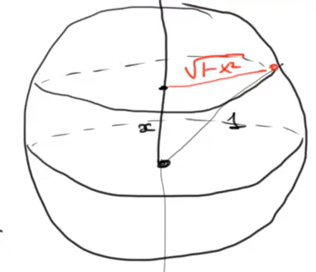
\includegraphics[width=7cm]{assets/03-intergrals-with-params/volume-of-n-dim-sphere.png}
            \end{center}

            $V_n(1) = \int_{-1}^{1} {V_{n - 1} \left( \sqrt{1 - x^2} \right) dx} = 2 \cdot \int_{0}^{1} { V_{n - 1} \left(\sqrt{1 - x^2}\right) dx } = 2 \cdot \int_{0}^{1} { \left(1 - x^2\right)^{\frac{n-1}{2}} \cdot C_{n-1} dx } \underbrace{=}_{x = \sin(\phi)}$
            
            $= 2 \cdot C_{n - 1} \cdot \int_{0}^{\frac{\pi}{2}} { \left(\cos^2(\phi)\right)^{\frac{n - 1}{2}} \cdot \cos(\phi) d \phi } = 2 C_{n - 1} \int_{0}^{\frac{\pi}{2}} { \cos^n(\phi) d\phi } = 2 C_{n - 1} \cdot \frac{1}{2} \cdot \frac{\Gamma\left(\frac{n+1}{2}\right)}{\Gamma\left(\frac{n+2}{2}\right)} \cdot \sqrt{\pi}$.

            Получили, что $C_n = C_{n - 1} \cdot \frac{\Gamma\left(\frac{n+1}{2}\right)}{\Gamma\left(\frac{n+2}{2}\right)} \cdot \sqrt{\pi}$.

            $C_n = \frac{\Gamma\left(\frac{n+1}{2}\right)}{\Gamma\left(\frac{n+2}{2}\right)} \cdot \sqrt{\pi} \cdot C_{n - 1} = \frac{\sqrt{\pi} \cdot \Gamma\left(\frac{n+1}{2}\right)}{\Gamma\left(\frac{n+2}{2}\right)} \cdot \frac{\sqrt{\pi} \cdot \Gamma\left(\frac{n}{2}\right)}{\Gamma\left(\frac{n+1}{2}\right)} \dots \frac{\sqrt{\pi} \cdot \Gamma\left(\frac{3}{2}\right)}{\Gamma\left(\frac{4}{2}\right)} C_1 = $

            $= 2 \cdot \frac{(\sqrt{\pi})^{n - 1} \cdot \Gamma\left(\frac{3}{2}\right)}{\Gamma\left(\frac{n}{2} + 1\right)} = \frac{\pi^{\frac{n-1}{2}} \Gamma\left(\frac{1}{2}\right)}{\Gamma\left( \frac{n}{2} + 1 \right)} = \frac{\pi^{\frac{n}{2}}}{\Gamma\left( \frac{n}{2} + 1 \right)}$.
        }
    \end{enumerate}
\end{example}

\Subsection{Криволинейные интегралы}

\begin{definition}
    $\gamma: [a, b] \to \mathbb{R}^n$ -- гладкая кривая

    $f$ -- функция, заданная на $\gamma[a, b] \to \mathbb{R}$

    Криволинейный интеграл ($I$ рода (интеграл по длине дуги)): 

    $\int_{\gamma}^{}fds := \int_{a}^{b}f(\gamma(f))\cdot ||\gamma'(t)||dt$, где $||\gamma'(t)|| = ||\begin{pmatrix}
        \gamma_1'(t)\\
        \gamma_2'(t)\\
        \vdots\\
        \gamma_n'(t)
    \end{pmatrix}|| = \sqrt[]{(\gamma_1'(t))^2 + \dots + (\gamma_n'(t))^2}$
\end{definition}

\begin{theorem}
    \begin{enumerate}
        \item Не зависит от параметризации кривой
        \item Не зависит от направления
        \item $\int_{\gamma}^{}ds = l(\gamma)$ -- длина кривой 
        \item Линейность по функции
        % todo: picture here
        \item Аддитивность по кривой: если $\gamma = \gamma_1 \sqcup \gamma_2$, то $\int_{\gamma}^{}f ds = \int_{\gamma_1}^{}f ds + \int_{\gamma_2}^{}f ds$
        \item Если $f \leq g$, то $\int_{\gamma}^{}f \leq \int_{\gamma}^{}g$
        \item $|\int_{\gamma}^{}f ds| \leq \int_{\gamma}^{}|f|ds$
        \item $\int_{\gamma}^{}fds \leq \max f \cdot l(\gamma)$
    \end{enumerate}
\end{theorem}

\begin{proof}
    \begin{enumerate}
        \item[1-2] $\tilde{\gamma}$ -- другая параметризация. $\tilde{\gamma} = \gamma \circ \tau$, где $\tau: [c, d] \to [a, b]$ -- гладкая строго монотонная биекция

        $\int_{\tilde{\gamma}}^{}f ds = \int_{c}^{d}f(\gamma(\tau(u)))||\tilde{\gamma'}(u)||du$

        $\tilde{\gamma'}(u) = \begin{pmatrix}
            \tilde{\gamma_1'}(u) \\
            \vdots
        \end{pmatrix}$

        $\tilde{\gamma_1} = \gamma_1 \circ \tau, \tilde{\gamma_1}'(u) = \gamma_1'(\tau(u))\tau'(u)$

        $||\tilde{\gamma}'(u)|| = |\tau'(u)| \cdot ||\gamma'(\tau(u))||$ -- если бы не было модуля, могли бы просто сделать замену переменной, но надо что-то умнее

        Если $\tau \uparrow$, тогда $\int_{a}^{b}f(\gamma(t)) \cdot ||\gamma'(t)|| dt = \int_{\gamma}^{}f ds$, где $t = \tau(u)$

        А если $\tau \downarrow$, то лишний минус появится, когда поменяем местами концы

        В итоге не зависим от убывания/возрастания

        \item[3] Формула для длины кривой
        \item[4] $\int_{\gamma}^{}(\alpha f + \beta g)ds = \int_{a}^{b}(\alpha f(\gamma(t))) + \beta g(\gamma(t))||\gamma'(t)||dt = \alpha \int_{a}^{b}f(\gamma(t))||\gamma'(t)||dt + \dots = \alpha \int_{\gamma}^{}f ds + \beta\int_{\gamma}^{}gds$
        \item[5] $\gamma: [a, b] \to \mathbb{R},\ c \in (a, b),\ \gamma_1 = \gamma|_{[a, c]}, \gamma_2 = \gamma|_{[c, b]}$ и по аналогии
        \item[6] $\int_{\gamma}^{}f ds = \int_{a}^{b}f(\gamma(t))||\gamma'(t)||dt$ и если заменим на $g$, станем только больше
        \item[7] $|\int_{\gamma}^{}f ds| = |\int_{a}^{b}f(\gamma(t))||\gamma'(t)||dt| = \int_{a}^{b}|f(\gamma(t))| \cdot ||\gamma'(t)||dt = \int_{\gamma}^{}|f|ds$
        \item[8] $f \leq \max f \implies \int_{\gamma}^{}fds \leq \int_{\gamma}^{}\max f ds = l(\gamma) \cdot \max f$
    \end{enumerate}
\end{proof}

\begin{remark}
    Можно определить $\int_{\gamma}^{}f ds$ для кусочно-гладких $\gamma$. Содержательная тут только проверка на корректность, но она проверятся с помощью аддитивности по кривой 
\end{remark}

% todo: change to "uprazhnenie" whatever this is
\begin{theorem}\textbf{Упражнение}

    $\int_{\gamma}^{}f ds = \lim \sum_{k = 1}^{m}f(\gamma(\xi(k))) \cdot l(\gamma|_[t_{k - 1}, t_k])$, где $\gamma: [a, b] \to \mathbb{R}^n$, при мелкости дробления $\to 0$
\end{theorem}

\begin{definition}
    Дифференциальная форма (1-го порядка) в $\mathbb{R}^n$

    $\omega = f_1dx_1 + f_2dx_2 + \dots + f_ndx_n$
\end{definition}

\begin{definition}
    Криволинейный интеграл $II$ рода (интеграл от дифференциальной формы)

    $\gamma: [a, b] \to \mathbb{R}^n$ -- гладкая кривая

    $\int_{\gamma}^{}\omega := \int_{a}^{b}(f_1(\gamma(t))\cdot\gamma_1'(t) + \dots + f_n(\gamma(t))\cdot\gamma_n'(t))dt$

    Если коротко: $\overline{f} = \begin{pmatrix}
        f_1\\
        f_2\\
        \vdots\\
        f_n
    \end{pmatrix}, \int_{\gamma}^{}\omega = \int_{a}^{b}\langle \overline{f}(\gamma(t)), \gamma'(t)\rangle dt$
\end{definition}

\begin{properties}
    \begin{enumerate}
        \item Не зависит от параметризации
        \item Смена направления меняет знак интеграла
        \item $\int_{\gamma}^{}\omega = \int_{\gamma}^{}\langle \overline{f}, \overline{\sigma} \rangle ds$, где $\overline{\sigma}$ -- единичный касательный вектор
        \item Линейность по $\overline{f}$
        \item Аддитивность по кривой
        \item $|\int_{\gamma}^{}\omega| \leq \int_{\gamma}^{}||\overline{f}||ds \leq \max ||\overline{f}|| \cdot l(\gamma)$
    \end{enumerate}
\end{properties}

\begin{proof}
    \begin{enumerate}
        \item $\tilde{\gamma} = \gamma \circ \tau, \tau : [c, d] \to [a, b]$ -- строго возрастает, гладкая, $\tau(c) = a, \tau(d) = b$.

        $\int_{\tilde{\gamma}}^{}\omega = \int_{c}^{d}\sum_{k = 1}^{n}f_k(\tilde{\gamma}'(u))du = \int_{c}^{d}\sum_{k = 1}^{n}f_k(\gamma(\tau(u)))\gamma_k'(\tau(u))\tau'(u)du = (*)$

        Делаем замену $t = \tau(u): (*) = \int_{a}^{b}\sum_{k = 1}^{n}f_k(\gamma(t))\gamma_k'(t)dt = \int_{\gamma}^{}\omega$

        \item Доказали вместе с первым: если меняется направление, то $\tau(c) = b, \tau(d) = a, \int_{b}^{a} = -\int_{\gamma}^{}\omega$

        \item $\overline{\sigma}(\gamma(t)) = \frac{\gamma'(t)}{||\gamma'(t)||}$. Тогда $\int_{\gamma}^{}\langle \overline{f}, \overline{\sigma} \rangle ds = \int_{a}^{b}\langle \overline{f}(\gamma(t)), \overline{\sigma}(\gamma(t)) \rangle ||\gamma'(t)|| dt = \int_{a}^{b} \langle \overline{f}(\gamma(t)), \frac{\gamma'(t)}{||\gamma'(t)||} \rangle||\gamma'(t)||dt = \int_{a}^{b} \langle \overline{f}(\gamma(t)), \gamma'(t) \rangle dt$
        \item[4, 5] следуют из 3
        \item[6] $|\int_{\gamma}^{}\omega| = |\int_{\gamma}^{} \langle \overline{f}, \overline{\sigma} \rangle ds| \leq \int_{\gamma}^{}|\langle \overline{f}, \overline{\sigma} \rangle| ds \leq \int_{\gamma}^{}||\overline{f}|| \cdot \overline{\sigma} || ds$
    \end{enumerate}
\end{proof}

%%todo: change to "uprazhnenie" whatever this is

\begin{theorem}\textbf{Упражнение}
    Доказать формулу: $\int_{\gamma}^{}\omega = \lim \sum_{j = 1}^{m} \sum_{k = 1}{n} f_k (\gamma(\xi_j))(\gamma_k(t_j) - \gamma_k(t_{j - 1}))$, если мелкость дробления $\to 0$

    $\gamma: [a, b] \to \mathbb{R}^n$
    
    %todo: picture here
\end{theorem}

\begin{definition}
    $\omega$ -- дифференциальная форма, заданная в $\Omega \subset \mathbb{R}^n$ -- открытом множестве

    $F: \Omega \to \mathbb{R}$ - первообразная для $\omega$, если $dF = \omega$

    $dF = \frac{\delta F}{\delta x_1}dx_1 + \dots + \frac{\delta F}{\delta x_n}dx_n$, т.е нужно, чтобы $\frac{\delta F}{\delta x_k} = f_k$ при $k = 1, 2, \dots, n$
\end{definition}

\begin{theorem}
    Пусть $F$ -- первообразная, $\omega$, $\gamma$ -- кривая, соединяющая точки $A, B$

    Тогда $\int_{\gamma}^{}\omega = F(B) - F(A)$
\end{theorem}

\begin{proof}
    $\gamma: [a, b] \to \mathbb{R}^n, f_k = \frac{\delta F}{\delta x_k}$

    $\int_{\gamma}^{}\omega = \int_{a}^{b}\sum_{k = 1}^{n}f_k(\gamma(t))\gamma_k'(t) dt = \int_{a}^{b}\underbrace{\sum_{k = 1}^{n} \frac{\delta F}{\delta x_k}(\gamma(t)) \cdot \gamma_k'(t)}_{(F \circ \gamma)'(t)} dt = \int_{a}^{b}(@F \circ \gamma)'(t) dt = F \circ \gamma(b) - F \circ \gamma(a) = F(\gamma(b)) - F(\gamma(a))$
\end{proof}

\begin{definition}
    $\Omega$ -- область, если $\Omega$ -- открытое линейно связанное множество

    Линейная связность -- любая пара точек может быть соединена какой-либо кривой $\in \Omega$
\end{definition}

\begin{consequence}
    \begin{enumerate}
        \item Если у $\omega$ есть первообразная, то $\int_{\gamma}^{}\omega$ зависит только от концов кривой, но не зависит от самой кривой
        \item Если $\Omega$ -- область, то все первообразные отличаются друг от друга на $\texttt{const}$
    \end{enumerate}
\end{consequence}

\begin{proof}
    2. \item $F$ и $G$ -- первообразные $\omega$, возьмем точки $A, B$ из $\Omega$ и соединим кривой $\gamma \implies G(B) - G(A) = \int_{\gamma}^{}\omega = F(B) - F(A) \implies G(B) = F(B) + G(A) _ F(A)$ (фиксируем $A$ и меняем $B$)
\end{proof}

\begin{lemma}
    $\Omega$ -- область $\implies$ между любыми двумя её точками можно провести ломанную, все звенья которой параллельны осям координат

    %todo: picture here
\end{lemma}

\begin{proof}
    $A, B \in \Omega \implies \exists \gamma: [a, b] \to \Omega$ такая что $\gamma(a) = A, \gamma(b) = B$. Для $t \in [a, b]$ рассмотрим шар $B_{r(t)}(\delta(t)) \in \Omega$
    
    %todo: picture here

    $\gamma[a, b]$ -- компакт $\implies$ выберем конечное подпокрытие. Тогда можем перемещаться между центрами шариков по звеньям, параллельным осям координат

    %todo: picture here
\end{proof}

\begin{theorem}
    Пусть $\Omega$ -- область, $\omega = f_1dx_1 + \dots + f_ndx_n$ -- дифференциальная форма в $\Omega$ и $f_1, f_2, \dots, f_n: \Omega \to \mathbb{R}$ -- непрерывные функции. Тогда следующие условия равносильны

    \begin{enumerate}
        \item $\omega$ имеет первообразную $F: \Omega \to \mathbb{R}$
        \item $\int_{\gamma}^{}\omega = 0$ для любой замкнутой кривой $\gamma$
        \item $\int_{\gamma}^{}\omega = 0$ для любой замкнутой ломаной $\gamma$ со звеньями, параллельными осям координат
    \end{enumerate}
\end{theorem}

\begin{proof}
    $1) \implies 2) \implies 3)$ очевидны

    $3) \implies 1)$: 

    %todo: picture here
    Соединим $c$ и $x \in \Omega$ ломаной со звеньями, параллельными осям координат. 
    
    $F(x) := \int_{\gamma}^{}\omega$. Поймем, что результат не зависит от выбора ломаной $\gamma$

    $0 = \int_{\gamma \cup \tilde{\gamma}^{-1}}^{}\omega = \int_{\gamma}^{}\omega + \int_{\tilde{\gamma}^{-1}}^{}\omega = \int_{\gamma}^{}\omega - \int_{\tilde{\gamma}}^{}\omega$, где $\tilde{\gamma}^{-1}$ -- инвертированная по направлению вторая ломаная

    Осталось проверить, что $\frac{\delta F}{\delta x_k} = f_k$

    % todo: picture here
    $\frac{\delta F}{\delta x_1}(x) = \lim_{h \to 0} \frac{F(x_1 + h, x_2, \dots, x_n) - F(x_1, \dots, x_n)}{h} = \lim_{h \to 0} \frac{-\int_{\gamma}^{}\omega + \int_{\gamma \sqcup [x, x + h]}^{}\omega}{h} = \lim_{h \to 0} \frac{1}{n}\int_{[x, x + h]}^{}\omega = \underbrace{=}_{[0, h] = [x, x + h] (\text{сдвиг на x})} \lim_{h \to 0} \frac{1}{n}\int_{0}^{h}\underbrace{f_1(\gamma(t))}_{x + e_1t}\underbrace{\gamma_1'(t)}_{= 1}dt = \lim \frac{1}{n}\underbrace{\int_{0}^{1}f_1(x + e_1t)dt}_{= h \cdot f_1(x + e_1h\cdot\theta, \theta \in (0, 1))} = f_1(x)$, т.к. $\gamma(t) = x + e_1 \cdot t, \gamma_1'(t) = 1, \gamma_2'(t) = \dots = \gamma_n'(t) = 0$
\end{proof}

\begin{remark}
    Для $\mathbb{R}^2$ 3) можно заменить на 3'): $\int_{\gamma}^{}\omega = 0$ для любого прямоугольного $\gamma$ со сторонами, параллельными осям координат
\end{remark}

\begin{proof}
    % todo: picture here
    Картинка.
\end{proof}

\begin{remark}
    $\omega$ в $\Omega \in \mathbb{R}^n$. В каждой точке $\Omega$ своё линейное отображение $\mathbb{R}^n \to \mathbb{R}$

    $\omega = f_1dx_1 + f_2dx_2 + \dots + f_ndx_n$

    $dx_1$ - функция $g_1(x) = x_1$

    $dg_1$

    $g_1(x + h) = g_1(x) + dg_1(g) = o(h)$, поэтому $dx_i$ в определении $\omega$ -- проекции на соотв. координаты
\end{remark}

\begin{definition}
    Живём в $\mathbb{R}^2$. Назовём элементарной область в $\mathbb{R}^2$, если 

    $\Omega = \{ (x, y) : a < x < b \texttt{and} \phi(x) < y < \psi(x) \} = \{ (x, y): c < y < d \texttt{and} \alpha(y) < x < \beta(y) \}$

    % todo: picture here
    Может показаться, что такого не бывает, но вот пример: *картинка*
\end{definition}

\begin{theorem}\textbf{Формула Грина}
    $\Omega \subset \mathbb{R}^2$ область, граница которой состоит из конечного числа кусочно гладких простых замкнутых кривых, ориентированных положительно

    $P, Q: Cl \Omega \to \mathbb{R}$ непрерывны, $\frac{\delta P}{\delta x}$ и $\frac{\delta Q}{\delta y}$ непрерывны 

    Тогда $\int_{\delta \Omega}^{}Pdx + Qdy = \int_{\Omega}^{}(\frac{\delta Q}{\delta y} - \frac{\delta P}{\delta x}dx) d\lambda_2$

    направление на кусочках границ такое, что область слева.

    % todo: picture here
    Ориентация устроена так: *картинка*
\end{theorem}
\begin{proof}
    $\int_{\Omega} { \frac{\delta Q}{\delta x} d \lambda_2 } = \int_{\delta \Omega} {Q dy}$ и $-\int_{\Omega} {\frac{\delta P}{\delta y} d \lambda_2} = \int_{\delta \Omega} {P dx}$

    \begin{enumerate}
        \item {
            % TODO: picture
            $\Omega$ -- элементарная область.

            $\int_{\Omega} {\frac{\delta P}{\delta y}} = \int_{a}^{b} { \int_{\phi(x)}^{\psi(x)} {\frac{\delta P}{\delta y} (x, y) dy} dx} = \int_{a}^{b} { P(x, \psi(x)) - P(x, \phi(x)) dx } = \int_{a}^{b} { P(x, \psi(x)) dx } - \int_{a}^{b} { P(x, \phi(x)) dx }$

            % TODO: make romanian numbers here instead of `(i)`
            $\int_{\delta \Omega} { P dx } = (1) + (2) + (3) + (4)$

            $x\rightarrow (x, \phi(x)): \ (1) = \int_{a}^{b} { P(x, \phi(x)) dx}$

            $y \rightarrow (b, y): \ (2) = \int_{\phi(b)}^{\psi(b)} { P(b, y) b' dy } = 0$

            $x \rightarrow (x, \psi(x)): \ (3) = -\int_{a}^{b} { P(x, \psi(x)) dx}$

            $y \rightarrow (a, y): \ (4) = - \int_{\phi(a)}^{\psi(x)} { P(a, y) a' dy } = 0$
        }
        \item {
            % TODO: picture
            Пусть для $\Omega_1$ и $\Omega_2$ ф-ла доказана, тогда $\int_{\Omega_i} { \left( \frac{\delta  Q}{ \delta x} - \frac{\delta P}{\delta y} \right) d\lambda_2 } = \int_{\delta \Omega_i} { P d x + Q dy } \implies \int_{\Omega_1} { \left( \frac{\delta  Q}{ \delta x} - \frac{\delta P}{\delta y} \right) d\lambda_2 } + \int_{\Omega_2} { \dots } = \int_{\delta \Omega_1} { Pdx + Qdy } + \int_{\delta \Omega_2} { \dots } = \int_{\delta \Omega} { P d x + Q d y } = \int_{\Omega} { \left( \frac{\delta  Q}{ \delta x} - \frac{\delta P}{\delta y} \right) }$.
        }
        \item {
            Формула верна для конечного объединения элем. областей.
        }
        \item {
            Скипнули? Что?
        }
    \end{enumerate}
\end{proof}
\begin{consequence}
    $\lambda_2 \Omega = \int_{\delta \Omega} { xdy } = - \int_{\delta \Omega}{y d x} = \frac{1}{2} \int_{\delta \Omega} { xdy - ydx }$
\end{consequence}


\Subsection{Точные и замкнутые формы}
\begin{definition}
    $\Omega$ -- область, $\omega$ -- дифф. форма в $\Omega$. $\omega$ -- точная форма, если у нее существует первообразная.
\end{definition}
\begin{definition}
    $\omega$ -- локально точная форма, если $\forall a \in \Omega$ найдется $U_a$, такая что в $U_a$ есть первообразная $\omega$.
\end{definition}
\begin{definition}
    $\omega = f_1 d x_1 + f_2 d x_2 + \dots + f_n d x_n$ -- замкнутная, если $\forall i, j: \ \frac{\delta f_i}{\delta x_j} = \frac{\delta f_j}{\delta x_i}$.
\end{definition}

\begin{remark}
    Точность $\implies$ локальная точность (но не наоборот).

    $\mathbb{R}^2 \setminus \{( 0, 0 )\}$.

    $\omega = \frac{x dy - y dx}{x^2 + y^2}$ не точная.

    $\int_{\text{един. окр.}} { \omega } = \int_{0}^{2\pi} { \frac{\cos(t) (\sin(t))' - \sin(t) (\cos(t))'}{\cos^2(x) + \sin^2(x)} dt} = \int_{0}^{2\pi} { dt } = 2\pi \not = 0$.

    $x = \cos(t), \ y = \sin(t)$.

    В верхней полуплоскости $F(x, y) = -\arctan\left(\frac{x}{y}\right)$ -- первообразная.

    $\frac{\delta F}{\delta x} = - \frac{\frac{1}{y}}{1 + (\frac{x}{y})^2} = \frac{y}{x^2 + y^2}$

    $\frac{\delta F}{\delta y} = - \frac{-\frac{x}{y^2}}{1 + (\frac{x}{y})^2} = \frac{x}{x^2 + y^2}$
\end{remark}

\begin{theorem}
    Если коэфф. из $C^1$, тогда локальная точность $\implies$ замкнутость.
\end{theorem}
\begin{proof}
    Берем $a \in \Omega$ и $U_a$, где есть первообразная $F \implies f_i = \frac{\delta F}{\delta x_i}$.

    $\frac{\delta f_i}{\delta x_j} = \frac{\delta}{\delta x_j} (\frac{\delta F}{\delta x_i}) = \frac{\delta^2 F}{\delta x_j \delta x_i} \underbrace{=}_{\text{т.к. непрер. слева и справа от равенства}} \frac{\delta^2 F}{\delta x_i \delta x_j} = \frac{\delta}{\delta x_i} \left( \frac{\delta F}{\delta x_j} \right) = \frac{\delta f_j}{\delta x_i}$.
\end{proof}

\begin{lemma}
    \textbf{Пуанкаре}.

    Если $\Omega$ -- выпуклая область и коэфф. формы из $C^1$, то замкнутость $\implies$ точность.
\end{lemma}
\begin{proof}
    Только для $\mathbb{R}^2$.

    Для существования первообр. достаточно чтобы интеграл по любому прямоугольнику со сторонами параллельными осям координат был равен 0.
    
    $\omega = P dx + Q dy: \ \int_{\text{обход контура}} { \omega } = \int_{\text{заполенные прямоуг.}} { (\frac{\delta Q}{\delta x} - \frac{\delta P}{\delta y}) d \lambda_2} = 0$.
\end{proof}

\begin{consequence}
    \begin{enumerate}
        \item {
            Замкнутая форма с коэфф. из $C^1$ в любом открытом шаре из $\Omega$ имеет первообразную.
        }
        \item {
            Замкнутая форма с коэфф. из $C^1$ лок. точная.
        }
    \end{enumerate}
\end{consequence}
\begin{definition}
    $\omega$ -- лок. точная форма в $\Omega$.

    $\gamma: \ [a, b] \rightarrow \Omega$ путь.

    $f: \ [a, b] \rightarrow \mathbb{R}$ первообразная $\omega$ вдоль пути $\gamma$, если $\forall t \in [a, b]$ у $\gamma(t)$ найдется окр. $U_{\gamma(t)}$, а в ней первообразная $F$ формы $\omega$, т.ч. $f(\tau) = F(\gamma(\tau))$ при $\tau$ близких к $t$.
    % TODO: picture
\end{definition}

\begin{theorem}
    Первообразная вдоль пути существует и единственная с точностью до константы.
\end{theorem}
\begin{lemma}
    Локально постоянная функция (в каждой точке есть окрестность, что функция на ней постоянная) -- константа.
\end{lemma}
\begin{proof}
    Док-во теоремы.

    \textbf{Единственность}: $f_1, \ f_2$ -- первообр. вдоль пути $\gamma$.

    $f_1 - f_2$ -- лок. постоянная, покажем это:

    Берем $t \in [a, b]$, есть $U_{\gamma(t)}$ и в ней первообр. $F_1$ и $F_2$, т.ч. $f_1(\tau) = F_1(\gamma(\tau))$ и $f_2(\tau) = F_2(\gamma(\tau))$ при $\tau$ близких к $t$, но $F_1 - F_2 = const \implies f_1 - f_2 = const$ при $\tau$ близких к $t$.


    \textbf{Существование}: берем $t \in [a, b]$, у $\gamma(t)$ есть окр-ть $U_{\gamma(t)}$, в которой существ. первообр.
    
    % TODO: picture

    $\bigcup_{t \in [a, b]} { U_{\gamma(t)} }$ -- покрытие $\gamma [a, b]$ -- компакт.

    Выберем конечные подпокрытия $U_1, \dots, U_m$ и $F_1, \dots, F_m$ -- первообр. в соотвествующем $U_j$.

    Из леммы Лебега $\exists r > 0: \ \forall t \in [a, b]: \ B_r(\gamma(t))$ целиком содержится в какаом-то эл-те покрытия.

    Нарежем $[a, b]$ на кусочки длины $< \delta$, где $\delta > 0$ выбрано по $\epsilon = r$ из равномерной непрерывности $\gamma$.

    %  TODO: picture

    $a =: t_0, t_1, \dots, t_n := b$ -- нарезка.

    Тогда образы маленьких отрезков целиком содержатся в своих элементах покрытия.

    $\delta [t_{i-1}, t_i] \subset U_i$, так занумеруем $F_i$ --- первообр. в $U_i$.

    $f|_{[t_0, t_1]} = F_1 \circ \gamma$, $f|_{[t_1, t_2]} = F_2 \circ \gamma$.

    В $\underbrace{U_1}_{\ni \gamma(t_1)} \cap U_2 \not = \emptyset \implies$ $F_1, F_2$ -- первообр. $\implies$ они отличаются на $const \implies F_2 = F_1 + c$, подменяем $c$ так, что в $U_1 \cap U_2$ они совпали. И так далее для всех остальных кусочков.
\end{proof}

\begin{consequence}
    $f$ -- первообраз. $\omega$ вдоль пути $\gamma: [a, b] \rightarrow \Omega$. Тогда $\int_{\gamma} {\omega} = f(b) - f(a)$
\end{consequence}
\begin{proof}
    % TODO: picture
    Смотрим на нарезку из предыдущей теоремы. Тогда $\int_{\gamma} {\omega} = \sum_{i=1}^{n} { \int_{\gamma|_{[t_{i - 1}, t_i]}} {\omega}} = \sum_{i=1}^{n} { \left( F_i(\gamma(t_i)) - F_{i}(\gamma(t_{i - 1})) \right) } = F_n(\gamma(b)) - F_1(\gamma(a)) = f(b) - f(a)$.

    $F_i(\gamma(t_i)) = F_{i + 1} (\gamma(t_i))$ так согласованы $F_j$.
\end{proof}

\begin{definition}
    $\Omega$ -- область в $\mathbb{R}^2$.

    $\gamma_0, \ \gamma_1: [a, b] \rightarrow \Omega$ пути в $\Omega$.

    \begin{enumerate}
        \item {
            $\gamma_0(a) = \gamma_1(a)$ и $\gamma_0(b) = \gamma_1(b)$.

            $\gamma_0, \gamma_1$ - гомотопные пути с неподвижными концами, если $\exists \gamma: [a, b] \times [0, 1] \rightarrow \Omega$ непрерывное, т.ч. $\forall t: \ \gamma(t, 0) = \gamma_0(t), \ \gamma(t, 1) = \gamma_1(t)$ и $\forall u: \ \gamma(a, u) = \gamma_0(a), \ \gamma(b, u) = \gamma_0(b)$.
            
            $\gamma_u (t) := \gamma(t, u)$ путь, соединяющий точки $\gamma_0(a)$ и $\gamma_0(b)$.

            % TODO: picture and another picture
        }
        \item {
            $\gamma_0(a) = \gamma_0(b), \ \gamma_1(a) = \gamma_1(b)$.

            $\gamma_0, \gamma_1$ -- гомотопно замкнутые пути, если $\exists \gamma: [a, b] \times [0, 1] \rightarrow \Omega$ непрерывное, т.ч. $\forall t : \ \gamma(t, 0) = \gamma_0(t), \ \gamma(t, 1) = \gamma_1(t)$ и $\forall u: \ \gamma(a, u) = \gamma(b, u)$.

            % TODO: picture
        }
    \end{enumerate}
\end{definition}
\begin{definition}
    $\gamma$ -- стягиваемы замкнутый путь в $\Omega$, если он гомотопен точке.
\end{definition}
\begin{definition}
    $\Omega$ -- односвязная область, если любой замкнутый путь в ней -- стягиваемый. 
\end{definition}
\begin{example}
    \begin{enumerate}
        \item {
            Выпуклая область односвязна (для любых двух точке верно, что отрзок, соединяющий их лежит в области).
            % TODO: picture
        }
        \item {
            Звездная область односвязна (одна точка фиксированна и верно, что отрезок соединяющий ее и любую другую лежит в области).
            % TODO: picture
            \begin{proof}
                $\Omega$ -- звездная, $O$ -- фикс. точка.

                $\gamma_1: [a, b] \rightarrow \Omega$ -- замк. путь.

                $\gamma_u(t) := u \cdot \gamma_1(t) \in \Omega$.

                $\gamma_0(t) = 0$.

                Хз, что это доказывает, но вот оно есть :/
            \end{proof}
        }
        \item {
            $\mathbb{R}^2 \setminus \{ (0, 0) \}$ не явл. односвязной.
        }
    \end{enumerate}
\end{example}

\begin{exerc}
    $\Omega$ -- односвязна, $f: \underbrace{\mathbb{T}}_{\text{окр. единичного радиуса}} \rightarrow \Omega$ непрер. отображ.

    Доказать, что существует $g: \text{замк. круг. един. радиуса} \rightarrow \Omega$ -- непрер.
\end{exerc}

\begin{definition}
    $\gamma: [a, b] \times [c, d] \rightarrow \Omega$ непрер. отображ.
    
    $\omega$ -- лок. точная форма в $\Omega$.

    $\forall (t, u) \in [a, b] \times [c, d]$ существует окр-ть $U_{\gamma(t, u)}$ и первообр $F$ в этой окр-ти, т.ч. $f(\tau, \nu) = F(\gamma(\tau, \nu))$.
\end{definition}

\begin{theorem}
    Первообразная отн-но отображения существует и единственна с точностью до константы.
\end{theorem}
\begin{proof}
    
    \textbf{Единственность}: $f, g$ -- первообразные отн-но отображения $\gamma$, то $f - g$ -- локально постоянная функция двух переменных $\implies f - g = const$.

    \textbf{Существование}: берем $(t, u) \in [a, b] \times [c, d]$, у $\gamma(t, u)$ есть окр-ть $U_{\gamma(t, u)}$ в которой существует первообразная $\implies [a, b] \times [c, d] \subset \bigcup_{(t, u) \in [a, b] \times [c, d]} {U_{\gamma(t, u)}}$.
    
    Выбираем конечное подпокрытие, по нему $r > 0$ из леммы Лебега $\implies B_r(\gamma(t, u))$ целиком содержится в эл-те подпокрытия.
    
    $\gamma \in C\left( [a, b] \times [c, d] \right) \implies $ равном. непрер. Берем по $\epsilon = r$ такое $\delta > 0$ из равн. непрерывности $\implies$ если $(t, u)$ и $(t', u')$ на расстоянии $< \delta$, то $\gamma(t, u)$ и $\gamma(t', u')$ на расстоянии $< r$.

    % TODO: picture
    $\gamma([t_{i - 1}, t_i] \times [u_{j - 1}, u_j]) \subset U_{ij}$ и $F_{ij}$ первообразная в $U_{ij}$.

    $f|_{[t_0, t_1] \times [u_0, u_1]} = F_{11} \circ \gamma$
    
    $f|_{[t_1, t_2] \times [u_0, u_1]} = F_{21} \circ \gamma$

    $\gamma(\{ t_1 \} \times [u_0, u_1]) \subset U_{11} \cap U_{21} \leftarrow$ тут $F_{11}, \ F_{21}$ -- первообраз. $\implies$ они отличаются на $const$.

    Подправим $F_{21}$ так, что в $U_{11} \cap U_{21}$ они совпадают.

    В итоге построим $f_1: [a, b] \times [c, d] \rightarrow \mathbb{R}$ -- первообр. отн-но $\gamma|_{[a, b] \times [u_0, u_1]}$.

    Аналогично $f_j: [a, b] \times [u_{j - 1}, u_j] \rightarrow \mathbb{R}$ -- первообр. онт-но $\gamma|_{[a, b] \times [u_{j - 1}, u_j]}$.

    осталось склеить их в $f$.

    Рассмотрим $f_1, \ f_2$. $f_1(\cdot, u_1), \ f_2(\cdot, u_1)$ -- первообр. вдоль пути $\gamma_{u_1} \implies$ они отличаются на константу.

    Подправим $f_2$ так, что $f_1(\cdot, u_1) = f_2(\cdot, u_1)$.

    % TODO: picture
\end{proof}

\begin{theorem}
    $\gamma_0, \gamma_1$ -- гомотопные пути с неподвижными концами в $\Omega$. $\omega$ -- локально точная форма в $\Omega$. Тогда $\int_{\gamma_0} {\omega} = \int_{\gamma_1} {\omega}$.
\end{theorem}
\begin{proof}
    $\gamma: [a, b] \times [0, 1] \rightarrow \Omega$ гомотопия между $\gamma_0, \gamma_1$.
    
    $f$ -- первообразная $\omega$ относительно отображения $\gamma$, $f(\cdot, 0)$ -- первообразная вдоль пути $\gamma_0$.

    $\int_{\gamma_0} {\omega} = f(b, 0) - f(a, 0)$.

    $\int_{\gamma_1} {\omega} = f(b, 1) - f(a, 1)$.
    
    Докажем, что $f(a, \cdot)$ -- лок. постоянная. Рассмотрим $(a, u)$: у $\gamma(a, u)$ есть окр-ть $U$ и в ней первообразная $F$, т.ч. $f(\tau, \nu) = F(\gamma(\tau, \nu))$ при $(\tau, \nu)$ близких к $(a, u)$.

    $f(a, \nu) = F(\gamma(a, \nu)) = F(\gamma_0(a))$ не зависит от $\nu$ (по аналогии делаем с другим концом и мы решили задачу. Но почему?! я хз).
\end{proof}

\begin{theorem}
    $\gamma_0, \ \gamma_1$ -- замкнутые гомотопные пути в $\Omega$. $\omega$ -- локю точная форма в $\Omega$. Тогда $\int_{\gamma_0} { \omega } = \int_{\gamma_1} { \omega }$.
\end{theorem}
\begin{proof}
    $\gamma: [a, b] \times [0, 1] \rightarrow \Omega$ -- гомотопия, $f$ -- первообразная $\omega$ относительно $\gamma$.

    $\int_{\gamma_0} { \omega } = f(b, 0) - f(a, 0)$
    
    $\int_{\gamma_1} { \omega } = f(b, 1) - f(a, 1)$

    Докажем, что $f(b, \cdot) = f(a, \cdot)$ лок. постоянна.
    
    Рассмотрим $(a, u)$, у $\gamma(a, u)$ есть окр-ть $U$ и в ней первообраз. $F$, т.ч. $f(\tau, \nu) = F(\gamma(\tau, \nu))$ при $(\tau, \nu)$ близких к $(a, u)$.

    Рассмотрим $(b, u)$, у $\gamma(b, u)$ есть окр-ть $\tilde{U}$ и в ней первообраз. $\tilde{F}$, т.ч. $f(\tau, \nu) = \tilde{F}(\gamma(\tau, \nu))$ при $(\tau, \nu)$ близких к $(b, u)$.

    $\gamma(a, u) = \gamma(b, u) \in U \cap \tilde{U}$

    $F$ и $\tilde{F}$ -- первообразные в $U \cap \tilde{U} \implies \tilde{F} = F + C$ в $U \cap \tilde{U}$.

    $f(b, \nu) - f(a, \nu) = \tilde{F}(\gamma(b, \nu)) - F(\gamma(a, \nu)) = \tilde{F}(\gamma(a, \nu)) - F(\gamma(a, \nu)) = C$.
\end{proof}

\begin{consequence}
    Если $\gamma_1$ -- стягивемый путь в $\Omega$, $\omega$ -- лок. точная форма в $\Omega$. Тогда $\int_{\gamma_1} {\omega} = 0$ю
\end{consequence}

\begin{theorem}
    Если $\Omega$ -- односвязна, а $\omega$ -- лок. точная, то $\omega$ -- точная.
\end{theorem}
\begin{proof}
    $\gamma_1$ -- замкнутая кривая $\implies \gamma_1$ -- стягиваемая $\implies \int_{\gamma_1} {\omega} = 0 \implies$ существует первообр.
\end{proof}

\begin{remark}
    $\mathbb{R}^2 \setminus \{ (0, 0) \}$ не односвязна, т.к. там есть лок. точная форма, не являющаяся точной.
\end{remark}

